\documentclass{article}
\usepackage[left=3cm, right=2.5cm, top=2cm]{geometry}
\usepackage{amsmath, amsthm, amssymb}
\usepackage{graphicx}
\usepackage[round]{natbib}
\usepackage{hyperref}
\usepackage{algorithm}
\usepackage[noend]{algpseudocode}

\makeatletter
\def\BState{\State\hskip-\ALG@thistlm}
\makeatother
\newcommand{\INDSTATE}[1][1]{\State\hspace{#1\algorithmicindent}}

\newtheorem{theorem}{Theorem}

% The line below tells R to use knitr on this.
%\VignetteEngine{knitr::knitr}

\title{An R Implementation for Correlated Pseudo Marginal Monte Carlo Methods}
\author{James Thornton \and Yuxi Jiang}

\usepackage{Sweave}
\begin{document}
\Sconcordance{concordance:cpmmc.tex:cpmmc.Rnw:%
1 22 1 1 0 251 1 1 2 1 0 1 2 1 0 2 1 1 3 1 0 1 8 6 0 1 4 2 0 1 4 2 0 1 %
4 2 0 1 5 3 0 1 12 9 0 1 3 1 0 1 1 3 0 1 2 2 1}


\maketitle

\begin{abstract}
This document briefly summarises the statistical methodology underlying the \texttt{cpmmc} package, located at \url{https://github.com/JTT94/cpmmc}. In particular, this paper looks at the Correlated Pseudo Marginal Markov Chain theory introduced by \cite{cpmmDeligiannidis2015} and application to the random effects model.
\end{abstract}

\section{Background}

The Metropolis-Hastings (MH) algorithm, detailed fully by \cite{roberts2004}, is a particular Markov Chain Monte Carlo (MCMC) procedure used to sample asymptotically from a target distribution, $\pi$, in order to compute expectations with respect to the target distribution. This and similar MCMC procedures are often employed when it is difficult to sample from $\pi$ directly. The outline of MH is that one builds a Markov chain with states $\{\theta_t ; t \in \mathbb{N}\}$, and stationary distribution $\pi$, coinciding with the desired target distribution. At each time $ t $ , the state is updated stochastically via an acceptance/rejection probability on a proposal state, $\theta^\prime$, generated from some transition kernel, $K$ with density $q$. The acceptance probability is defined as  $ \alpha_E(\theta_{t-1}, \theta^\prime) = min\left\{1,  \frac{
                \pi(\theta^\prime) q(\theta^\prime, \theta_{t-1})}
                {\pi(\theta_{t-1}) q(\theta_{t-1}, \theta^\prime)}
\right\} $. Provided certain ergodic conditions given by \cite{roberts2004} hold, the arithmetic average of accepted states in the generated Markov Chain will approach the desired expectation with respect to $\pi$. \\

In a Bayesian context, MH is often used to sample from a posterior distribution of some parameter of interest, $\theta$. Given observations $y_{1:T}$, and parameter of interest with prior distribution $p$, the target distribution will be of the form $\pi (\theta) = p(\theta | y_{1:T} ) \propto p(y|\theta) p(\theta)$.\\

To implement MH for Bayesian inference, one would need to be able to evaluate $p(y|\theta) p(\theta)$ in order to perform the acceptance/rejection step in building the Markov chain. For many applications, such as with latent variable models, the likelihood, $ p(y | \theta)$, is often intractable thus making MH difficult to implement. \\

The pseudo-marginal (PM) algorithm follows the same procedure as the idealised MH, however, it introduces an estimator for the intractable likelihood to replace the true likelihood ratio required for the acceptance probability. This reduces the requirement of being able to compute likelihood $p(y|\theta)$, to only being required to be able to compute a non-negative, unbiased, unnormalised Monte Carlo estimate of this likelihood. \\

The correlated pseudo-marginal (CPM) algorithm is a development of the PM algorithm and shall be the focus of this document. The CPM correlates the estimators for the likelihood to reduce the variance of the resulting likelihood ratio, in order to improve efficiency in implementing the scheme. In \cite{cpmmDeligiannidis2015}, correlated auxiliary variables are introduced in the calculation of the likelihood estimate to encourage correlation in the estimates.\\

The main contributions of \cite{cpmmDeligiannidis2015}, in addition to introducing this correlation approach, are: providing theoretical results on the benefits, guidance on tuning parameters and demonstrated applications in state space and random effect models. This document shall focus on the high-level CPM theory, random effect model and a simulation study to demonstrate some properties empirically.

\section{Methodology}
Let $p(y_{1:T}|\theta)$ denote the likelihood for the $T$ observations $y_{1:T}$, and let $p(\theta)$ be the prior density for the parameter $\theta \in \Theta \subseteq \mathbb{R}^{d}$. The Bayesian posterior density of interest can be written as $\pi (\theta) \propto p(y_{1:T}|\theta) p(\theta)$. To further abuse notation, let $x \sim p$ denote sampling realisation x from the distribution with density $p$.\\

\subsection{Metropolis-Hastings}
In a Bayesian setting, the MH algorithm is as detailed below, the acceptance probability has been rewritten from $\alpha_E(\theta_{t-1}, \theta^\prime) = min\left\{1,  \frac{
                \pi(\theta^\prime) q(\theta^\prime, \theta_{t-1})}
                {\pi(\theta_{t-1}) q(\theta_{t-1}, \theta^\prime)}\right\}$ to
 $ \alpha_E(\theta_{t-1}, \theta^\prime) = min\left\{1,  \frac{
                p(y_{1:T}| \theta^\prime) q(\theta^\prime, \theta_{t-1})p(\theta^\prime)}
                {p(y_{1:T}| \theta_{t-1}) q(\theta_{t-1}, \theta^\prime)p(\theta_{t-1})}
\right\} $ to emphasis the need to compute the exact likelihood.

\begin{algorithm}[H]
\caption{Idealised Metropolis Hastings}\label{euclid}
\begin{algorithmic}[1]
\BState  $\text{Initialise } \theta_0 :$ \newline
\indent \text{Sample from prior} \hspace{\algorithmicindent} $\theta_0 \sim p$
\BState  $\text{At each iteration } t>0:$
\State \hspace{\algorithmicindent} $\text{Sample proposal: }$
$\theta^\prime \sim q(\theta_{t-1}, \cdot)$
\State \hspace{\algorithmicindent} $\text{Calculate acceptance probability } \alpha_E(\theta_{t-1}, \theta^\prime):$ \newline
\centerline{
 $ \alpha_E(\theta_{t-1}, \theta^\prime) = min\left\{1,  \frac{
                p(y_{1:T}| \theta^\prime) q(\theta^\prime, \theta_{t-1})p(\theta^\prime)}
                {p(y_{1:T}| \theta_{t-1}) q(\theta_{t-1}, \theta^\prime)p(\theta_{t-1})}
\right\} $} \newline
\State \hspace{\algorithmicindent} $\text{With probabiliy: } \alpha_E(\theta_{t-1}, \theta^\prime)$ \newline \centerline{$\text{Set } \theta_t \gets \theta^\prime \text{ else } \theta_t \gets \theta_{t-1} $}
\end{algorithmic}
\end{algorithm}


\subsection{Correlated Pseudo-Marginal Algorithm} \label{cpm}
To target $\pi$, the CPM first augments the state from $\theta$ to $(\theta, U)$, with joint density $\bar{\pi}$ given as:
$$\bar{\pi}(\theta, u) = \pi(\theta)m(u)\frac{\hat{p}(y_{1:T}| \theta, u)}{p(y_{1:T}| \theta)}$$
By simulating a Markov chain to target $\bar{\pi}$, one can record only the $\theta$ values in order to target $\pi$. Given that $\hat{p} (y_{1:T} | \theta, U)$ is unbiased, we have that $\pi(\theta)$ is a marginal density of $\bar{\pi} (\theta, u)$, as $\int \bar{\pi}(\theta,u)du = \pi(\theta)$. \\

The Correlated Pseudo Marginal algorithm uses the following assumptions, as well as the Metropolis Hastings algorithm to target $\bar{\pi}$ with a choice of transition kernel $K$ to induce correlated $U$ proposals.
\begin{itemize}
 \item $\hat{p}(y_{1:T}| \theta, U)$ is a non-negative, unbiased estimator of likelihood $p(y_{1:T}| \theta)$
 \item $U \sim m$
 \item $K$ is a transition kernel admitting an m-reversible Markov chain $$ m(u)K(u,u^\prime) = m(u^\prime)K(u^\prime, u)$$
\end{itemize}


This framework allows for running MH without having to compute $p(y_{1:T}| \theta)$. The primary difference to the idealised MH algorithm is swapping the likelihood ratio, $\frac{ p(y_{1:T}| \theta, U^\prime)}{ p(y_{1:T}| \theta, U)}$, with its estimator $\frac{ \hat{p}(y_{1:T}| \theta, U^\prime)}{ \hat{p}(y_{1:T}| \theta, U)}$ in the acceptance probability at each iteration. \\

Informally, the intuition behind the CPM, and in particular the correlation aspect, is as follows. Providing $\hat{p}(y_{1:T}| \cdot, \cdot)$ as a function of $(\theta, U)$ is sufficiently `nice' and $\theta$ is close to $\theta^\prime$, correlation amongst $U$ and $U^\prime$ will induce correlation amongst $\hat{p}(y_{1:T}| \theta, U)$ and $\hat{p}(y_{1:T}| \theta^\prime, U^\prime)$. This correlation lowers the variance of the ratio seen in the acceptance probability, $\frac{ \hat{p}(y_{1:T}| \theta, U^\prime)}{ \hat{p}(y_{1:T}| \theta, U)}$. Hence, the algorithm will be `more similar' to the idealised MH algorithm, and reduce the inefficiency introduced by taking estimates rather than computing the exact values of the likelihood.


\begin{algorithm}[H]
\caption{Correlated Pseudo Marginal Algorithm}\label{euclid}
\begin{algorithmic}[1]
\BState  $\text{Initialise }  :$ \newline
\indent \hspace{\algorithmicindent} $\theta_0 \sim p_\theta$ \newline
\indent  \hspace{\algorithmicindent} $U_0 \sim p_U$
\BState  $\text{At each iteration } t>0:$
\State \hspace{\algorithmicindent} $\text{Sample proposal: }$
$\theta^\prime \sim q(\theta_{t-1}, \cdot)$
\State \hspace{\algorithmicindent} $\text{Sample auxiliary variables: }$
$ \epsilon \sim \mathcal{N}(0_M, I_M)$ \newline
\indent \text{Set } $U^\prime = \rho U_{t-1} + \sqrt{1-\rho^2} \epsilon$
\State \hspace{\algorithmicindent} $\text{Compute estimator } \hat{p}(y_{1:T}| \theta^\prime, U^\prime) \text{ of } p(y_{1:T}| \theta^\prime, U^\prime)$
\State \hspace{\algorithmicindent} $\text{Calculate acceptance probability: } \alpha_E(\theta_{t-1}, \theta^\prime):$ \newline
\centerline{
 $ \alpha_E\{(\theta_{t-1}, U_{t-1}), (\theta^\prime, U^\prime)\} = min\left\{1,  \frac{
                \hat{p}(y_{1:T}| \theta^\prime, U^\prime) q(\theta^\prime, \theta_{t-1})p(\theta^\prime)}
                {\hat{p}(y_{1:T}| \theta_{t-1}, U_{t-1}) q(\theta_{t-1}, \theta^\prime)p(\theta_{t-1})}
\right\} $} \newline
\State \hspace{\algorithmicindent} $\text{With probabiliy: } \alpha_E\{(\theta_{t-1}, U_{t-1}), (\theta^\prime, U^\prime)\}$ \newline
\centerline{$\text{Set } (\theta_t, U_t) \gets (\theta^\prime, U^\prime) \text{ else } (\theta_t, U_t) \gets (\theta_{t-1}, U_{t-1}) $}
\end{algorithmic}
\end{algorithm}

Notice that by setting $K(u, u\prime) = m(u \prime)$ and letting $\rho = 0$ in the CPM algorithm given above, we will obtain the PM algorithm.

\subsection{Random Effect Model}

Define the model as follows:
\begin{align}
x \sim& f_\theta(\cdot) \\
Y_t| X_t \sim& g_\theta(\cdot | X_t)
\end{align}
where $t \in \mathbb{N}$ and $\{X_t; t>0\}$ are $\mathbb{R}^k$-valued latent variables and $\{Y_t; t>0\}$ are $\mathcal{Y}$-valued observations.\\

For observed data $Y_{1:T}=y_{1:T}$, the likelihood satisfies:
\begin{align}
p(y_{1:T})=& \prod_{t=1}^{T} p(y_t|\theta) \\
p(y_t| \theta)=& \int g_\theta(y_t|x_t,\theta)f_\theta(x_t) dx_t
\end{align}

If the integral for $p(y_t| \theta)$ is intractable, one can use importance sampling to form an unbiased estimator $\hat{p}(y_t| \theta)$, where $N$ is the number of proposal samples. The likelihood estimator and importance sampling weights are given by:

\begin{align}
\hat{p}(y_{1:T}| \theta, U) =& \prod_{t=1}^{T} \hat{p}(y_t|\theta, U_t) \\
\hat{p}(y_t| \theta, U_t)=& \frac{1}{N} \sum_{i=i}^N w(y_t, U_{t,i}; \theta ) \\
w(y_t, U_{t,i}) =& \frac{g_\theta(y_t|X_{t,i})f_\theta(X_{t,i})}{q_\theta(X_{t,i}|y_t)}
\end{align}
assuming that there exists a deterministic map $ \Xi: \mathbb{R}^p \times \Theta \rightarrow \mathbb{R}^k$ such that $X_{t,i} = \Xi(U_{t,i}, \theta) \sim q_\theta(\cdot|y_t)$ and $U_{t,i} \sim \mathcal{N}(0_p, I_p) $.

\subsection{Key Results on Parameter Tuning and Optimisation} \label{norm_dist}

Other than introducing the approach, the primary theoretic contributions of \cite{cpmmDeligiannidis2015} are in specifying the distributions of the loglikelihood error, $Z_T(\theta)$, and loglikelihood error ratio, $R_T(\theta, \theta^\prime)$ under correlated $U$ proposals and under non-correlated for comparison of CPM with the PM algorithm.

\begin{align}
Z_T(\theta) =& \log(\hat{p}(Y_{1:T}| \theta, U)) - \log(p(Y_{1:T}|\theta))\label{eq:Z} \\
R_T(\theta, \theta^\prime) =& \log \frac{\hat{p}(Y_{1:T}| \theta^\prime, U^\prime)}{\hat{p}(Y_{1:T}| \theta, U)} - \log \frac{p(Y_{1:T}| \theta^\prime,)}{p(Y_{1:T}| \theta)} \label{eq:R}
\end{align}

The significance of these results lies in using them to inform choice of parameters $\rho$ and $N$ which controls the correlation and number of Monte Carlo samples in the unbiased estimator respectively. \\

In the interest of brevity, the theorems of \cite{cpmmDeligiannidis2015} which state that $Z_T(\theta)$ and $R_T(\theta, \theta^\prime)$ are asympototically normal are not repeated below. However, the key practical implications are that one should find $\beta>0, \psi>0$ and set the CPM parameters such that:

\begin{align}
N_T =& \beta T ^{\frac{1}{2}} \label{eq:n}\\
\rho =& \exp(-\psi \beta T ^ {-\frac{1}{2}}) = \exp(-\psi \frac{N_T}{T}) \label{eq:rho}
\end{align}

\cite{cpmmDeligiannidis2015} then provides a heuristic to find these parameters by minimizing the objective function $CT(h, Q_T)$, detailed below.

\begin{align}
CT(h, Q_T) =& N_T \times IF(h, Q_T) \\
IF(h, Q_T) =& 1 + 2 \sum_{n=1}^{\infty} \phi_n (h, Q_T) \label{eq:IF}
\end{align}


Let $h$ be some real-valued measurable function. $IF(h, Q_T)$ is a measure of the integrated autocorrelation time of $\{h(\theta_t) ; t \in \mathbb{N}\}$, where $\{\theta_t\}_{t \in \mathbb{N}}$ are generated under Markov kernel $Q_T$. For $n>0$, $\phi_n$ denotes the autocorrelation at lag $n$. Thus, $IF(h, Q_T)$ provides a measure for inefficiency, and can be used to compare mixing performances between MCMC procedures. \\

Due to the involved nature, the detailed analysis of the heuristic has been excluded from this document.


  \section{Application}

  \subsection{Simulation Study}
  In order to compare the performance of CPM algorithm with PM and MH algorithms, we first introduce the following Gaussian random effects model:

  \begin{align*}
  X_t &\overset{\text{i.i.d.}}{\sim} N(\theta, 1) \\
  Y_t | X_t &\overset{\hphantom{\text{i.i.d.}}}{\sim} N(X_t, 1)
  \end{align*}

We also choose prior $\theta \sim \mathcal{N}(0,1)$. Under this particular construction, we can obtain the true likelihood $Y_t \sim N(\theta, 2)$, which not only can be used to directly implement the MH algorithm for benchmarking purposes, but also enables the computation of loglikelihood error and loglikelihood error ratio.\\

The three algorithms use the same random walk proposal distribution, $ \theta^\prime \sim \mathcal{N}(\theta, 0.02^2)$, where $0.02$ was chosen to coincide with \cite{cpmmDeligiannidis2015}. In addition, we use importance sampling to obtain a non-negative, unbiased estimator for the likelihood, given bellow, to compute the acceptance probabilities for the PM and CPM schemes.

\begin{align}
\hat{p}(y_{1:T}| \theta, U) =& \prod_{t=1}^{T} \hat{p}(y_t|\theta, U_t) \\
\hat{p}(y_t| \theta, U_t)=& \frac{1}{N} \sum_{i=i}^N \psi (y_t; \theta + U_{t,i}, 1)
\end{align}
where $\psi(\cdot; \mu, \sigma^2)$ denotes the density for the Gaussian distribution with mean $\mu$ and variance $\sigma^2$, and the auxilary variables $U_{t,i}$ are realisations from independent standard Gaussian distributions. \\

The true value for the `unknown' parameter of interest, $\theta$, is set to be $0.5$ when generating observations $y_{1:T}$.


\begin{figure}[H]
  \centerline{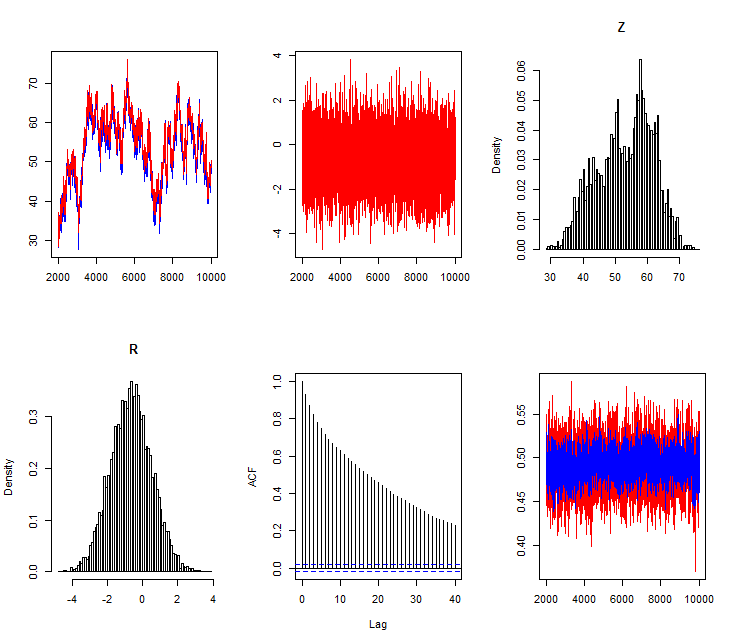
\includegraphics[scale=1]{experi1_plots}}
  \caption{Top row (left to right): Trace of $W_T$ (blue) and $Z_T$ (red) against iteration index; Trace of $R_T=W_T-Z_T$; histogram of $Z_T$.  Bottom row: Histogram of R, correlogram of acceptance chain for $\theta$; trace of accepted $\theta$ (blue) vs proposed (red). Where $Z_T$ and $R_T$ are as defined in \eqref{eq:Z} and \eqref{eq:R} and $W_T = \log(\hat{p}(Y_{1:T}| \theta^\prime, U^\prime)) - \log(p(Y_{1:T}|\theta^\prime))$. Data taken from case where $T=8192$ in table \ref{tab:table}}
  \label{fig:theFig}
\end{figure}

As seen by the figure \ref{fig:theFig}, $R_T$ empirically appears normal, as aluded to in section \ref{norm_dist}. $Z_T$ however, appears far from normally distributed, insinuating a possible lack of convergence or slow convergence.

\begin{figure}[H]
  \centerline{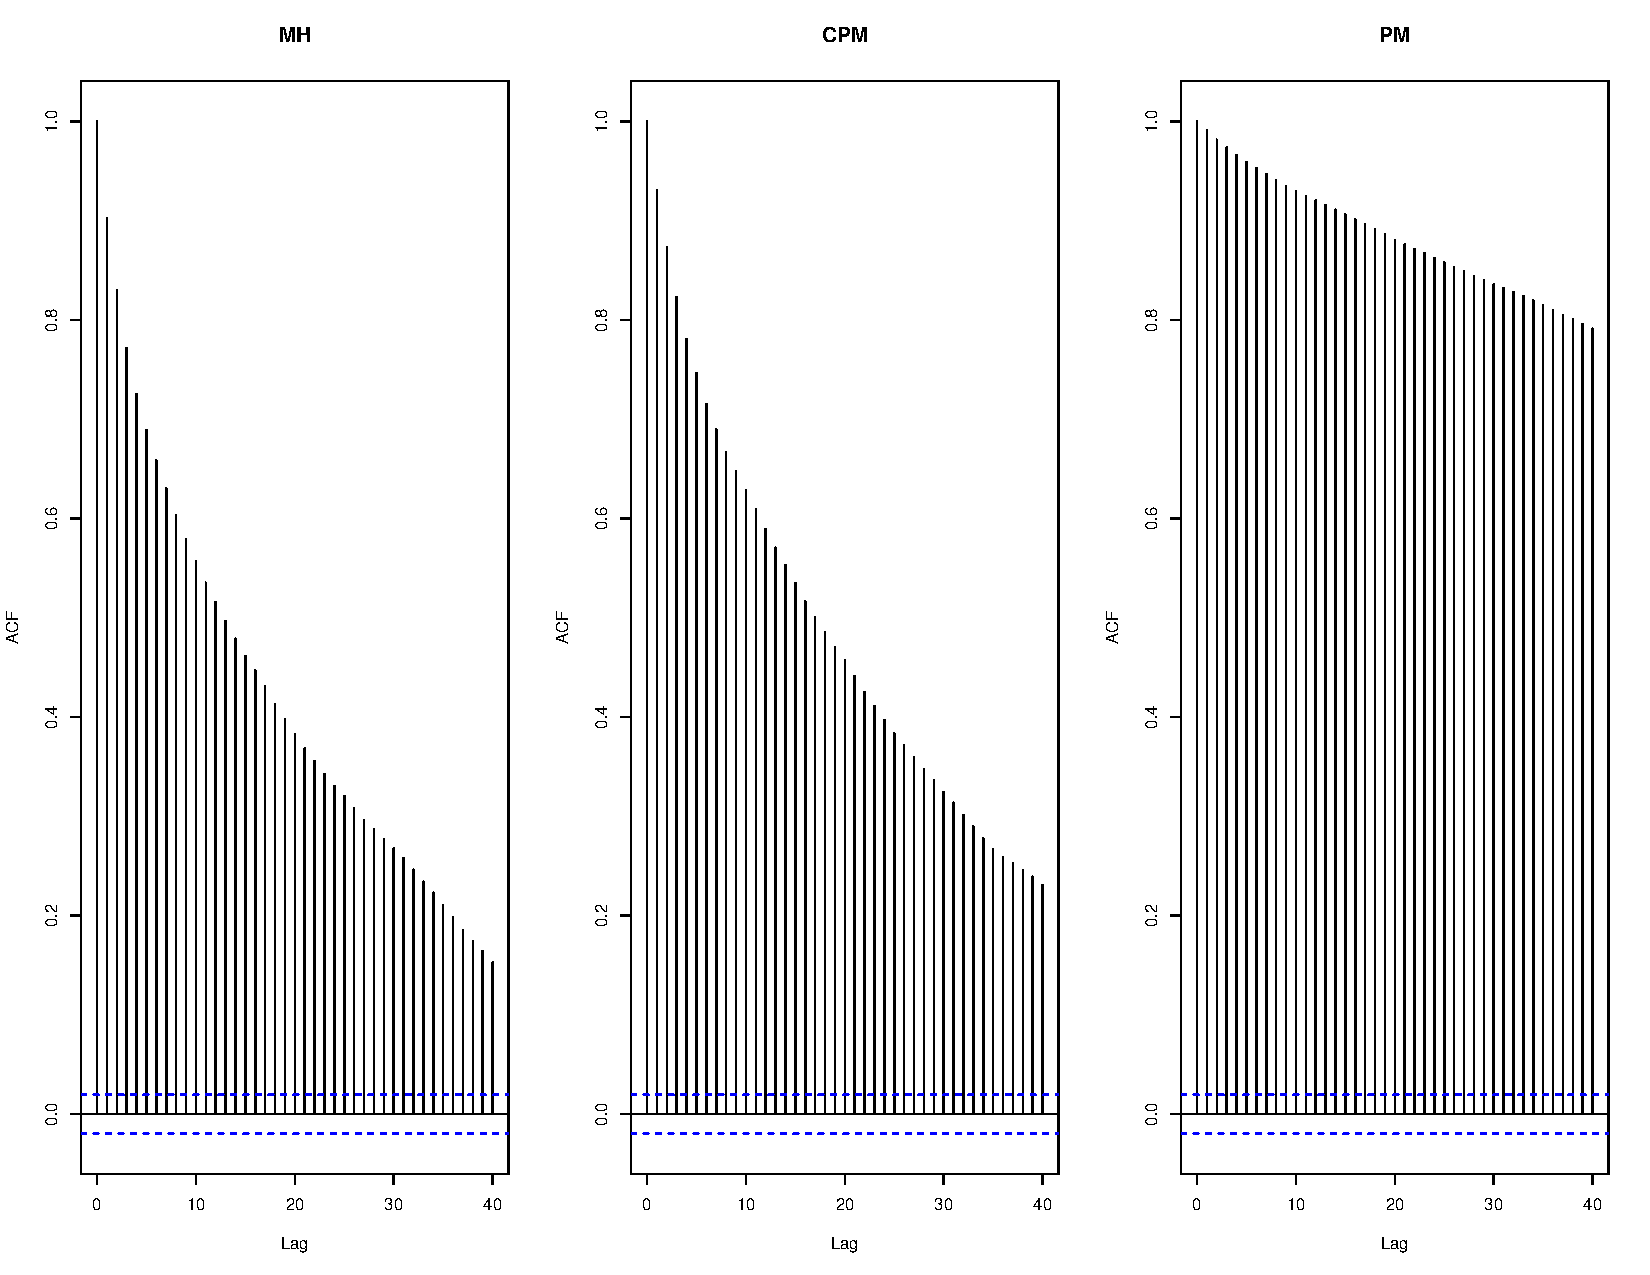
\includegraphics[scale=1]{acf_plots}}
  \caption{ACF plots for algorithms MH, CPM, PM. Data taken from case where $T=8192$ in table \ref{tab:table}}
  \label{fig:acf}
\end{figure}

As can be seen in the plot \ref{fig:acf}, correlation drops-off as lag is increased at a much higher rate using the CPM compared to PM algorithm, and again quicker in the MH. This would likely insinuate a faster exploration of the state-space, and faster convergence to the target distribution. If the chain remains in a trapped local area, then it would exhibit slowly decreasing autocorrelation. This is essentially what metric $IF$ \eqref{eq:IF} measures.

\subsection{Benchmarking: MH, CPM, PM}

Table \ref{tab:table} and table \ref{tab:RIF} detail multiple experiments with various data sizes, $T$, and tuned parameters $\rho$ and $N_T$ (tuned acording \eqref{eq:n} and \eqref{eq:rho}), across the 3 algorithms: CPM, PM and MH. The table clearly illustrates the higher average acceptance rate for MH over CPM and CPM significantly over PM, and indeed improved (lower) inefficiency scores. This clearly suggests that the CPM has noticable benefits over the PM in terms of efficient mixing of the chain, and comparable to the idealised MH in this toy example. It is still unclear whether these benefits would persist in higher dimensions. It is also certainly worth noting that the CPM algorithm took significantly longer to run than MH.

\begin{table}[H]
\centering
\begin{tabular}{|l|ll|lll|lll|}
\hline
     & \multicolumn{2}{l|}{} & \multicolumn{3}{l|}{Average Acceptance}           & \multicolumn{3}{l|}{Inefficiency Score, $h$} \\
$T$  & $N_T$     & $\rho$    & $\varrho_{MH}$ & $\varrho_{CPM}$ & $\varrho_{PM}$ & $IF_{MH}$     & $IF_{CPM}$    & $IF_{PM}$    \\ \hline
1024 & 19        & 0.9894    & 0.85           & 0.45            & 0.0052         & 18.78         & 27.04         & 78.95        \\
2048 & 28        & 0.9925    & 0.78           & 0.47            & 0.0044         & 11.96         & 21.65         & 76.56        \\
4096 & 39        & 0.9947    & 0.72          & 0.44            & 0.0040         & 11.91         & 20.54         & 53.66        \\
8192 & 80        & 0.9963    & 0.65           & 0.44            & 0.0031         & 19.92         & 24.34         & 64.29        \\ \hline
\end{tabular}
\caption{IF is defined by \eqref{eq:IF}, the where the sum is approximated up to lag 40 and $h(\theta)=\theta$, and $\varrho_{x}$ is the average acceptance rate for algorithm $x$. $N_T$ and $\rho$ have been chosen according to heuristic detailed in \cite{cpmmDeligiannidis2015}}
\label{tab:table}
\end{table}


\begin{table}[H]
\centering
\begin{tabular}{|l|ll|ll|}
\hline
     & \multicolumn{2}{l|}{} & \multicolumn{2}{l|}{Relative Inefficiency} \\
$T$  & $N_T$     & $\rho$    & $RIF_{CPM}$               & $RIF_{PM}$              \\ \hline
1024 & 19        & 0.9894    & 1.44                      & 4.2                     \\
2048 & 28        & 0.9925    & 1.81                      & 6.4                     \\
4096 & 39        & 0.9947    & 1.7                       & 4.5                     \\
8192 & 80        & 0.9963    & 1.2                       & 3.2                     \\ \hline
\end{tabular}
\caption{$RIF_x = IF_x/ IF_{MH}$ for algorithm $x$}
\label{tab:RIF}
\end{table}

  \section{Discussion}

As seen in the simulation study for the random effects model, the correlated pseudo marginal algorithm displays attractive peformance relative to the regular pseudo marginal algorithm. Additionally, the CPM has a lower requirement threshold, in terms of being able to compute the target density, than the idealised Metropolis Hastings and can be a candidate fitting algorithm in many cases where direct MH may not be possible, for example in latent variable models or non-conjugate random effect models. There are however limitations that must be stated.\\

  As mentioned informally Section \ref{cpm}, in order for correlated auxiliary variables, $U_t$, to induce correlated likelihood estimators, the estimator function $(\theta, U) \rightarrow \hat{p}(y | \theta, U)$ must be a `sufficiently regular' function. It may not however always be possible to fulfil this requirements. Indeed, \cite{cpmmDeligiannidis2015} used the particle-filter estimator for a state-space model as an example, as the likelihood ratio estimator does not behave as required even for `close' $(\theta, U)$ and $(\theta^\prime, U^\prime)$. In such cases, further steps may be required to make the CPM work, eroding efficiency. \cite{cpmmDeligiannidis2015} introduced a resampling scheme procedure based on the Hilbert space-filling curve and the `Particle filter using Hilbert sort' algorithm in order to sample from the state-space model, for example. \\

Similarly, \cite{cpmmDeligiannidis2015} induced correlation in normally distributed auxiliary variables, and required a deterministic mapping from these variables to the latent variables. Although not explored, this may be a cumbersome requirement. We imagine regular importance sampling would also work, however may be less efficient. \\

Although more efficient than the PM algorithm, the CPM can also be computationally expensive, and hence often time-consuming on a single machine. In the case of the random effects model, the CPM scheme requires one to simulate $N$ samples to compute a likelihood estimate using the importance sampling estimator for each observed data point, and this has to be repeated $T$ times to compute the acceptance probability for a single iteration. If the parameter of interest is of dimension $p$, then the CPM algorithm has to simulate $NTp$ random variables per iteration to get one sample, which can be expensive, especially if slow convergence requires many iterations. Per the recommendation, $N_T =T^{\frac{1}{2}}$, therefore the algorithm would run at $\mathcal{O}(T^{\frac{3}{2}})$. It is possible there are more competitive approximate methods.\\

One further comment is that the parameter tuning heuristic detailed by \cite{cpmmDeligiannidis2015} requires an initial model run. In practice, the suggested procedure is to evaluate $CT(h, Q_{T})$ only on a subset of data, then the parameters can be estimated through regression. However, multiple model runs may deteriorate performance when considered as a whole.\\

Future work may involve considering higher dimensional problems i.e. $p>1$, and parallelising the random effects model algorithm on the importance sampling step, which is the bottle-neck in the implementation.

  % now generate the bibliography from file mybib.bib
\bibliographystyle{plainnat}
\bibliography{mybib}

\section{Example code}
\begin{Schunk}
\begin{Sinput}
> library(cpmmc)
> # Initialise parameters ----
> T_ <- 100; N_ <- 5; rho <- 0.9963;
> nsim <- 10^4; burnin <- 100; theta_0 <- 0
> u_0 <- array(rnorm(T_*N_), dim = c(N_,1,T_))
> # Generate data and initialise ----
> data <- rnorm(T_,0.5, sd = sqrt(2))
> # Instantiate models ----
> # MH (class which class cpmmc inherits from)
> # For MH
> # --------------------------------
> log_target_density <- function(data, theta){
+   (sum(dnorm(data, mean = theta, sd = sqrt(2), log = T))) + dnorm(theta, log = T, sd = 1)
+ }
> log_target_density_theta <- function(theta){
+   log_target_density(data, theta)
+ }
> proposal_sampler <- function(state){
+   rnorm(1, mean = state, sd = 0.02)
+ }
> log_proposal_density <- function(state, proposal){
+   dnorm(proposal, mean = state, log=T, sd = 0.02)
+ }
> rem_mh <- metropolis_hastings(theta_0, # inital value
+                           log_target_density_theta,
+                           log_proposal_density,
+                           proposal_sampler)
> log_theta_prior_density = function(x) dnorm(x, log = T, sd = 1)
> log_theta_proposal_density = function(old_theta, new_theta)
+                               dnorm(new_theta-old_theta, log = T, sd=0.02)
> theta_proposal_sampler = function(x) rnorm(1, mean = x, sd = 0.02)
> # Random Effect CPM (specific case inherited from cpmmc class)
> rem_cpm <- normal_random_effect_model(data,
+             theta_0 = theta_0,
+             u_0 = u_0,
+             rho = rho
+ )
> # Run models for nsim iterations
> rem_cpm <- run_chain(rem_cpm, chain_length = nsim)
> rem_mh <- run_chain(rem_mh, chain_length = nsim)
\end{Sinput}
\end{Schunk}


  \end{document}
